\documentclass[twocolumn,10pt]{article}
\usepackage[margin=2cm]{geometry}

\usepackage[T1]{fontenc}
\usepackage[utf8]{inputenc}

\usepackage{graphicx}
\usepackage{hhline}

\usepackage{amsmath}
\usepackage{amssymb}
\usepackage{amsthm}

\newtheorem{proposition}{Proposition}

\usepackage[colorlinks=true]{hyperref}

\begin{document}

\title{Encoding SPAN Evolution Using Frequent-Collision Blockchains}
\author{Ryan Robinett and Tiago Royer}
\date{11 Dec 2019}
\maketitle

\begin{abstract}
	Blockchains are an implementation of a public distributed ledger,
	which allows for information to be agreed upon by several parties
	without the need of a central authority.
	When transposing the concept of blockchains to smartphone ad-hoc networks (SPANs),
	assumptions like relative stability of the underlying network are violated,
	which inevitably forces the blockchain to fork.
	In this context,
	instead of avoiding the creation of forks,
	we propose leveraging these long-term global forks
	as a way to record information about geographical proximity of the undelying SPAN.
	We present a simulation package for analyzing the forking behavior,
	alongside with a protocol for performing local geographical authentication
	based on this forking behavior.
\end{abstract}

\section{Introduction}

Geographical authentication
is the task of certify that someone is at a certain place;
that is,
the task of authenticating someone's geographical location.
This problem has been considered for over 20 years~\cite{denning_1996}.
The authors of \cite{denning_1996} consider the problem of finding
the location of an intruder;
other applications include geographically restricted broadcasts~\cite{gdpr},
checkins at Foursquare,
and withdrawing cash at an ATM.

In all these examples,
there is a central authority which confers authentication services.
Besides all the traditional problems with centralized solutions,
like having a single point of failure,
services like Foursquare have to essentially believe the user's word
when attesting they were at a certain place~\cite{glas2015breaking}.
ATM's circumvent this by essentially being a large network of totems,
which is expensive~\cite{totem_patent}.

The above solutions suffer from either having to trust too heavily upon
the user's word, or from implementing an expensive network of totems to
vet user dishonesty. The former makes a system unreliable, while the latter
imposes a startup cost that is not realistic for small players trying to enter
the market.

For reasons of decentralization and low cost, we would like a
means of local geographic authentication where users---each user represented as
a smartphone---mutually and simultaneously encode their geographic location using
handshakes with nearby users. In this work, we show that there exists a
blockchain-like distributed ledger protocol which, when implemented on top of some
smartphone ad hoc network (SPAN), encodes user geotemporal information strictly in
terms of the topology of that user's local blockchain. We further present a simulation
package which---unlike any preexisting package know to the authors---allows for the
simulation of a blockchain-like ledger system implemented over arbitrary SPAN
topologies.

\section{Motivation}
\label{sec:motivation}

Many smartphones today are equipped with wireless functionality specifically
geared towards interacting with other smartphones in near geographic proximity.
Assuming these connections faithfully represent one's geographic
authentication\footnote{This is an important problem which we do not attempt to
address in this paper. We are only concerned with whether a blockchain-like distributed
ledger implemented over a SPAN can reliably encode information about the SPAN's evolution
over time using nothing more than the topology of local copies of the blockchain.},
it follows immediately that, if each smartphone is a node $u$ connected to node $v$ if and only
if $u$ and $v$ are within interaction proximity---the set of neighbors of $u$ serves as
a valid representation of $u$'s geographic location. Further, if two nodes $u,v$ claim to be
in the same geographic location (given the location is sufficiently granular), it is expected
that the set of neighbors they report would significantly overlap. For this reason,
recording ``handshakes'' with peers in geographic proximity should serve as a valid
representation of one's location over time.

\subsection{Three Evolving Topologies: Implications of Blockchain over a SPAN}

The Bitcoin protocol is heavily dependent on a few assumptions concerning
the topology of the underlying network. While it relies on the fact that no
node can have global knowledge of what nodes are in the network due to the
ease with which nodes may enter and exit the network, it also assumes that the
network is stable enough to offer such features as never partitioning and never
being susceptible to man-in-the-middle attacks~\cite{nakamoto2008bitcoin}. This
relative stability is what allows all nodes in the network to asymptotically
agree on which blocks constitute the global blockchain. Further, this global
blockchain naturally arises as the set-theoretic intersection of all local 
chains in the network.

Implementing a blockchain system over a SPAN, however, breaks all of the
aforementioned assumptions. SPANs are highly volatile, and they can easily
partition into disconnected components. This makes the idea of nodes
globally converging to agreement on what is a global blockchain ridiculous, as
the intersection of all local blockchains would cease to grow as soon as
nodes disagree on which is the longest chain. It is guaranteed, however,
that for all nodes $u$ in the SPAN $G$, there exists some neighborhood
$U\subset G$ containing $u$ such that, if one takes the intersection
$$\mathbf{B}_U=\bigcup_{u^\prime\in U}\mathcal{B}_{u^\prime}$$
of all local blockchains $\mathcal{B}_{u^\prime}$ for all $u^\prime\in U$, 
it holds that $\mathbf{B}_U$ grows nontrivially for all timesteps\footnote{To 
	see that this is correct, it is sufficient to note that this trivially
	holds for $U=\{u\}$.}.

The degree to which all subsets $U\subset G$ satisfy this property is the
degree to which a global blockchain is well defined, and the degree to which
most subsets $U$ fail to do so can serve as a measure of the degree to which
a global blockchain is poorly defined. For this reason, the authors present
the idea of a \textit{semi-global blockchain}: the global blockchain with regards
to a connected subnetwork $U$ of the network $G$, as arises
as the set-theoretic intersection of all local chains $\mathcal{B}_u$ held by
nodes $u\in U$.

\begin{figure*}
	\centering
	\begin{tabular}{|p{2cm}||p{5cm}|p{1.5cm}|p{2.5cm}|p{3cm}|}
		\hline
		\ & \textbf{P2P Topology} & \textbf{Local Block-chain (per node)} & \textbf{Global Blockchain} & \textbf{Semi-Global Blockchain (per neighborhood)}\\
		\hhline{|=||=|=|=|=|}
		\textbf{Bitcoin P2P} 
			& The Bitcoin protocol relies on the assumption that
				no node in the underlying network can have
				complete global knowledge of the state of the
				network, especially given nodes can spontaneously enter or
				exit the network. However, it is also assumed that
				this network never becomes disconnected and never
				becomes vulnerable to man-in-the-middle attacks.
				In this way, it is safe to assume that all local
				nodes can eventually agree on some global state
				information.
			& Very similar, up to slight differences in protocol
			& The global blockchain is implicitly induced as the
				set-theoretic intersection of all local blockchains.
				It is guaranteed in probability that this intersection
				chain is always growing; failure to grow would imply
				that this global chain has forked.
			& For any connected subnetwork $G^\prime$ of the network, the
				global chain of the restriction to $G^\prime$ always
				(asymptotically) agrees with the well-defined global
				chain. \\
		\hline
		\textbf{SPAN P2P}
			& SPANs are highly volatile. The frequent making and
				breaking of connections causes the SPAN
				to fragment into disconnected components. It is hopeless,
				therefore, to assume that all the nodes will ever
				agree on global state information that is not
				granted \textit{a priori}.
			& Very similar, up to slight differences in protocol
			& Though the set-theoretic intersection of all local
				blockchains is well-defined, this intersection is
				likely to be noninteresting and stop growing after some
				timestep due to forking.
			& Let $G$ be the network. For each node $u\in G$, there exists
				neighborhoods $U,u\in U\subset G$ such that the global
				chain is well defined with respect to the restriction
				to $U$. We can define \textit{semi-global blockchains}
				as the intersection of local chains with respect to
				such restrictions. \\
		\hline
	\end{tabular}
	\caption{The Nakamoto paper assumes that the blockchain protocol is
		implemented over a relatively stable P2P network. If we attempt to
		implement a blockchain protocol over a SPAN, however, many of the
		notions that naturally arise in the case of Bitcoin no longer appear.
		The SPANchain simulator was written to allow for easy simulation of 
		blockchains implemented over SPANs, together with graphic tools which
		the authors hope helps the research community come up with ways
		of studying semi-global blockchains in the case of a forking global chain.}
	\label{tab:three_table}
\end{figure*}

Traditionally,
blockchain networks strive mantain a single longest path
starting from the root of the chain;
that is,
the goal is to avoid global forks.
In the case of Bitcoin,
for example,
local, temporary forking still happens
but one of those forks is usually quickly abandoned by the network~\cite{decker_2013}.
In our case,
since SPANs are often disconnected,
the global blockchain will eventually fork.
We actually embrace forking as a feature:
each long-term fork represents a connected component of the underlying SPAN.

\section{The SPANchain Simulator}
\label{sec:SPANchain}

We present a tool which allows for the simulation of the evolution of SPANs
---represented as random geometric graphs---over time, and which, most saliently,
allows for the simulation of a novel blockchain-like distributed ledger overlaid
on this SPAN. While the authors are aware of 1) network simulation tools that
accommodate dynamic network topologies~\cite{chaudhary2012study} and
2) tools for simulating blockchain
systems distributed over a network of nodes, we are unaware of any tool that
allows for the simulation of a blockchain system implemented over arbitrary dynamic
networks. Part of the reason for this is that SPANs, by nature, induce a network topology
that fragments easily and from which nodes enter and exit with great frequency. For
conventional blockchain systems, this inevitably leads to forking in the global
chain---a property which, for cryptocurrency applications, is highly undesirable
~\cite{decker_2013,nakamoto2008bitcoin}. Using our simulation tool, however, we show
that the way global forks form in blockchain networks implemented over SPANs can encode
geotemporal information about how the SPAN evolves over time.

In order to observe the behavior of this network under several scenarios,
we wrote a simulator package SPANchain%
\footnote{
	The code for the simulator is publicly available at
	\url{https://github.com/robbobbinett/geographic_auth_with_bc}.
}
for the protocol.

To the best of our knowledge,
this is the first blockchain simulation framework which simulates
blockchains implemented over SPANs, as well as the first
to embrace forking as a feature rather than a bug.
Therefore,
there are no packages which are capable of simulating a forking blockchain.
We also are not aware of any packages that implement blockchains over SPANs.

Although we implemented the protocol described in sections
\ref{sec:blockchain} in the simulator,
the package is written to be agnostic to the protocol for block formation,
as well as processes by which the underlying topology evolves\footnote{We have,
	however, implemented a class of SPAN-nodes to specifically handle
	the evolution of the SPAN with respect to a random geometric graph model.}.
We hope that these packages can be used by other researchers
to better understand how blockchains fork, and what information this forking
encodes with respect to the history of the underlying topology.


\section{Blockchains over SPANs}
\label{sec:motivation}

Many smartphones today are equipped with wireless functionality specifically
geared towards interacting with other smartphones in near geographic proximity.
Assuming these connections faithfully represent geographic proximity%
\footnote{
	Breaking this assumption is an important problem which we do not attempt to
	address in this paper. We are only concerned with whether a blockchain-like distributed
	ledger implemented over a SPAN can reliably encode information about the SPAN's evolution
	over time using nothing more than the topology of local copies of the blockchain.
},
it follows immediately that, if each smartphone is a node $u$ connected to node $v$ if and only
if $u$ and $v$ are within interaction distance---the set of neighbors of $u$ serves as
a valid representation of $u$'s geographic location. Further, if two nodes $u,v$ claim to be
in the same geographic location (given the location is sufficiently granular), it is expected
that the set of neighbors they report would significantly overlap. For this reason,
recording ``handshakes'' with peers in geographic proximity should serve as a valid
representation of one's location over time.

\subsection{Three Evolving Topologies: Implications of Blockchain over a SPAN}

The Bitcoin protocol is heavily dependent on a few assumptions concerning
the topology of the underlying network. While it relies on the fact that no
node can have global knowledge of what nodes are in the network due to the
ease with which nodes may enter and exit the network, it also assumes that the
network is stable enough to offer such features as never partitioning and never
being susceptible to man-in-the-middle attacks~\cite{nakamoto2008bitcoin}. This
relative stability is what allows all nodes in the network to asymptotically
agree on which blocks constitute the global blockchain. Further, this global
blockchain naturally arises as the set-theoretic intersection of all local 
chains in the network.

Implementing a blockchain system over a SPAN, however, breaks all of the
aforementioned assumptions. SPANs are highly volatile, and they can easily
partition into disconnected components. This makes the idea of nodes
globally converging to agreement on what is a global blockchain ridiculous, as
the intersection of all local blockchains would cease to grow as soon as
nodes disagree on which is the longest chain. It is guaranteed, however,
that for all nodes $u$ in the SPAN $G$, there exists some neighborhood
$U\subset G$ containing $u$ such that, if one takes the intersection
\begin{equation*}
	\mathbf{B}_U = \bigcap_{v \in U}\mathcal{B}_v
\end{equation*}
of all local blockchains $\mathcal{B}_v$ for all $v \in U$,
it holds that $\mathbf{B}_U$ grows nontrivially for all timesteps%
\footnote{
	To see that this is correct,
	it is sufficient to note that this trivially holds for $U=\{u\}$.
}.

The degree to which all subsets $U\subset G$ satisfy this property is the
degree to which a global blockchain is well defined, and the degree to which
most subsets $U$ fail to do so can serve as a measure of the degree to which
a global blockchain is poorly defined. For this reason, the authors present
the idea of a \textit{semi-global blockchain}: the global blockchain with regards
to a connected subnetwork $U$ of the network $G$, as arises
as the set-theoretic intersection of all local chains $\mathcal{B}_v$ held by
nodes $v \in U$.

\begin{figure*}[t]
	\centering
	\begin{tabular}{|p{3cm}||p{6.7cm}|p{6.7cm}|}
		\hline
		& \textbf{Bitcoin P2P} & \textbf{SPAN P2P} \\
		\hhline{|-||-|-|}

		\textbf{P2P Topology} &
			The Bitcoin protocol relies on the assumption that
			no node in the underlying network can have
			complete global knowledge of the state of the
			network, especially given nodes can spontaneously enter or
			exit the network. However, it is also assumed that
			this network never becomes disconnected and never
			becomes vulnerable to man-in-the-middle attacks.
			In this way, it is safe to assume that all local
			nodes can eventually agree on some global state
			information.
			&
			SPANs are highly volatile. The frequent making and
			breaking of connections causes the SPAN
			to fragment into disconnected components. It is hopeless,
			therefore, to assume that all the nodes will ever
			agree on global state information that is not
			granted \textit{a priori}.
			\\
		\hline

		\raggedright
		\textbf{Local Block-\\chain (per node)} & % Kludge, I know
			\multicolumn{2}{|l|}{
				Very similar, up to slight differences in protocol
			}
			\\
		\hline

		\textbf{Global Blockchain} &
			The global blockchain is implicitly induced as the
			set-theoretic intersection of all local blockchains.
			It is guaranteed in probability that this intersection
			chain is always growing; failure to grow would imply
			that this global chain has forked.
			&
			Though the set-theoretic intersection of all local
			blockchains is well-defined, this intersection is
			likely to be noninteresting and stop growing after some
			timestep due to forking.
			\\
		\hline

		\raggedright
		\textbf{Semi-Global Blockchain (per neighborhood)} &
			For any connected subnetwork $G^\prime$ of the network, the
			global chain of the restriction to $G^\prime$ always
			(asymptotically) agrees with the well-defined global
			chain.
			&
			Let $G$ be the network. For each node $u\in G$, there exists
			neighborhoods $U,u\in U\subset G$ such that the global
			chain is well defined with respect to the restriction
			to $U$. We can define \textit{semi-global blockchains}
			as the intersection of local chains with respect to
			such restrictions.
			\\
		\hline
	\end{tabular}
	\caption{The Nakamoto paper assumes that the blockchain protocol is
		implemented over a relatively stable P2P network. If we attempt to
		implement a blockchain protocol over a SPAN, however, many of the
		notions that naturally arise in the case of Bitcoin no longer appear.
		The SPANchain simulator was written to allow for easy simulation of 
		blockchains implemented over SPANs, together with graphic tools which
		the authors hope helps the research community come up with ways
		of studying semi-global blockchains in the case of a forking global chain.}
	\label{tab:three_table}
\end{figure*}

Traditionally,
blockchain networks strive mantain a single longest path
starting from the root of the chain;
that is,
the goal is to avoid global forks.
In the case of Bitcoin,
for example,
local, temporary forking still happens
but one of those forks is usually quickly abandoned by the network~\cite{decker_2013}.
In our case,
since SPANs are often disconnected,
the global blockchain will eventually fork.
We actually embrace forking as a feature:
each long-term fork represents a connected component of the underlying SPAN.


\section{The SPANchain Simulator}
\label{sec:SPANchain}

We present a tool which allows for the simulation of the evolution of SPANs
---represented as random geometric graphs---over time, and which, most saliently,
allows for the simulation of a novel blockchain-like distributed ledger overlaid
on this SPAN. While the authors are aware of 1) network simulation tools that
accommodate dynamic network topologies~\cite{chaudhary2012study} and
2) tools for simulating blockchain
systems distributed over a network of nodes, we are unaware of any tool that
allows for the simulation of a blockchain system implemented over arbitrary dynamic
networks. Part of the reason for this is that SPANs, by nature, induce a network topology
that fragments easily and from which nodes enter and exit with great frequency. For
conventional blockchain systems, this inevitably leads to forking in the global
chain---a property which, for cryptocurrency applications, is highly undesirable
~\cite{decker_2013,nakamoto2008bitcoin}. Using our simulation tool, however, we show
that the way global forks form in blockchain networks implemented over SPANs can encode
geotemporal information about how the SPAN evolves over time.

In order to observe the behavior of this network under several scenarios,
we wrote a simulator package SPANchain%
\footnote{
	The code for the simulator is publicly available at
	\url{https://github.com/robbobbinett/geographic_auth_with_bc}.
}
for the protocol.

To the best of our knowledge,
this is the first blockchain simulation framework which simulates
blockchains implemented over SPANs, as well as the first
to embrace forking as a feature rather than a bug.
Therefore,
there are no packages which are capable of simulating a forking blockchain.
We also are not aware of any packages that implement blockchains over SPANs.

Although we implemented the protocol described in sections
\ref{sec:blockchain} in the simulator,
the package is written to be agnostic to the protocol for block formation,
as well as processes by which the underlying topology evolves\footnote{We have,
	however, implemented a class of SPAN-nodes to specifically handle
	the evolution of the SPAN with respect to a random geometric graph model.}.
We hope that these packages can be used by other researchers
to better understand how blockchains fork, and what information this forking
encodes with respect to the history of the underlying topology.


\section{Adapting the Bitcoin Protocol}
\label{sec:blockchain}

\subsection{Exchanging Transactions for Handshakes}

Once a block is generated and published,
it is never removed from the local blockchain of a node recognizing
this block. The Bitcoin network ensures this feature with high
probability by forcing a child block to reference a pre-existing parent
block using a nonce $n$ which, together with a hashed parent ID $P$, satisfies
the inequality $H(n,P)<\tau$ for globally define hash function $H$ and
threshold value $\tau$~\cite{nakamoto2008bitcoin}.
This section formalizes how blocks are created and recognized by nodes in a SPAN
in the SPANchain module.

The blockchain is essentially a tree of blocks,
containing solutions to cryptographic challenges.
A \emph{cryptographic challenge} is a pair
\begin{equation*}
	\mathcal P = (t_C, k_C)
\end{equation*}
where $t$ is a timestamp and $k$ is the public key of the problem creator.
Each \emph{block} is, in turn, a tuple of the form
\begin{equation*}
	B = (t_C, k_C, t_S, k_S, n, b),
\end{equation*}
where $(t_C, k_C)$ form a cryptographic challenge,
$n$ is the nonce which solves the challenge (described below)
$k_S$ is the public key of the problem solver,
$t_S$ is the timestamp of when $n$ was found,
and $b$ is a pointer to a parent block.
Additionally,
the empty block $(\varnothing, \varnothing, \varnothing, \varnothing, \varnothing)$
is a valid block.
This is the global root of the blockchain tree.

We assume the existence of a cryptographically secure hash function $H$.
Denote by $t_c k_C k_S b$ the concatenation of $t_c$, $k_C$, $k_S$ and $b$.
A nonce $n$ is a \emph{solution} to the problem contained in a block $B$ as above
if $H(B) < \tau$,
where $\tau$ is a predefined threshold value known \emph{a priori} by the network.

\subsection{Rate of Block Formation as a Function of $\tau$}

Nakamoto's original paper discusses regulating the rate of block formation in
the global chain by
periodically updating the threshold $\tau$ for which all blocks
$B=(t_C, k_C, t_S, k_S, n, b)$ must satisfy $H(B)<\tau$~\cite{nakamoto2008bitcoin}.
Decker \textit{et al.} subsequently show that the rate at which block collisions
occur in the Bitcoin network can be modeled as a function of the rate of block
creation. Putting these together, we surmise that our rates of block formation
and global forking can be set arbitrarily high or low relative to the rates at
which changes occur in the topology of the underlying SPAN. This allows us to
simulate our peer-to-peer (P2P) message passing over the SPAN in such
a way that, given network churn is kept low, we can run SPAN updates and
block updates/propagation as discrete events that do not overlap or otherwise
interfere.

% TODO: add example


\section{Simulation}
% TODO

\subsection{SPAN Connectivity Model}

The protocol runs over an ad-hoc network,
where each node is a smartphone
and the nodes connect wirelessly to each other.
In the simulation,
we modelled this underlying infrastructure using a dynamic random graph.

The most commonly studied model of random graphs is the Erdős--Rényi model.
Given parameters $n$ and $p$,
the model generates a graph with $n$ vertices
and each edge is added to the graph independently with probability $p$~\cite{bollobas_2001}.
This model, however,
has no information about node positions,
which makes it a poor representative of ad-hoc networks~\cite{Hekmat2006}.

Instead,
we will use random geometric graphs as our connectivity model.
Given parameters $n$ and $r$,
the model randomly chooses $n$ points in the unit square $[0, 1]^2$,
uniformly and independently,
and adds an edge between each points which are at a distance $r$ from each other.
Random geometric graphs
have been proposed as accurate models for ad-hoc networks~\cite{Kenniche2010,Hekmat2006}.

Nodes which are close to the borders of the unit square
are affected by the so-called ``border effect'':
if the distance of a node is smaller than $r$
from any of the borders,
then part of the ``area of coverage'' for this node
(that is,
the area which may contain adjacent vertices)
lies outside of the unit square.
This effectively truncates the degree of that node,
because no nodes are generated outside the unit square.
For smaller values of $r$ this effect is less pronounced,
because less nodes are affected.

In order to avoid the border effect,
we will use toroidal distances instead~\cite{Kenniche2010,Hekmat2006}.
The nodes will be placed on the unit torus $[0, 1)^2$
and distances will be measured according to a toroidal metric.
So,
for example,
for $r = 0.1$,
the nodes at $(0.01, 0.01)$ and $(0.99, 0.99)$ are adjacent in this metric.

We will denote
the toroidal random geometric graph model with parameters $n$ and $r$
by $T(n, r)$.

We want to model the underlying infrastructure to be dynamic,
to represent the fact that nodes move around in the world.
That is,
we will have a sequence $G_0, G_1, \dots$ of graphs over the same set of nodes,
which represent the evolution of the network.

Using the toroidal has the benefit that
if the nodes move around randomly, but independently,
then each resulting graph is still a geometric graph.
More precisely,

\begin{proposition}
	Let $G_0 \in T(n, r)$ be a random graph.
	For each $i \in \mathbb N$,
	define $G_{i+1}$ by translating each vertex $v \in V(G_i)$
	by a random translation vector $u_v$,
	chosen independently according to some distribution,
	and connecting vertices which are within a distance of $r$ of each other.
	Then, for each $i$,
	the graph $G_i$ is a random geometric graph distributed according to $T(n, r)$.
\end{proposition}

Note that each $G_i$ will be distributed according to $T(n, r)$,
regardless of the distribution of the translation vectors $u_v$
(as long as each translation vector is chosen independently,
and irrespective of the vector $v$).

% TODO: Proof?

However,
there are little literature using several different translation parameters.
We will use a simplified version of the dynamic model of~\cite{Diaz2008}.
Fixed a parameter $s$,
$G_{i+1}$ is generated from $G_i$
by translating each vertex by a vector with norm $s$,
chosen uniformly among all $s$-normed vectors in $\mathbb R^2$.

% TODO: Picture?

\subsection{Visualizing the Interplay between Local and Semi-Global Chains}

Due to the SPANchain module existing for less than a quarter of a year, it
lacks a complete set of visualization tools for analyzing the
behavior of semi-global blockchains over SPANs. Partly, this is due to
our module being the first to accommodate forking as a feature rather than
a bug; the only degree to which forking is well-understood in the literature
is how one can best prevent it from happening. Though furthering our work
will require rigorous measures of semi-global blockchain formation and
diversity, we offer the following toy case as a proof of concept that the persistence of
semi-global chains in the network (i.e. the degree to which a non-trivial
global blockchain failes to exist) preserve information as to how the SPAN
topology has changed over time.

The top of Figure \ref{fig:old_town_road} shows a connected SPAN which maintains
its initial state long enough for ten blocks to form and propagate. The SPAN
then partitions into two connected components, remains in this state long enough for
ten more blocks to form and propagate, and finally reverts to its original state.
The simulation randomly grants and deterministically propagates ten more blocks before
terminating.

The bottom of Figure \ref{fig:old_town_road} shows the local blockchain held by a
specific node in the described SPAN. The local chain recognizes all blocks indices
zero through nine, as all problem formulations and blocks from all other nodes
reached the node in question. However, this node does not recognize all of blocks ten
through 19, as some of these were discovered by nodes in the other partition during the
period of disconnection. By the time the two partitions joined back together, we see two
branches in the local chain competing for status as global chain; one of these, which
begins with the edge from node zero to node 21, represents the continuation of what had
been the longest chain in the other partition. As half the nodes in the network recognize
it as the longest chain, leaves on this chain become parent references for roughly half
of the problem proposals created in the network. Though the branch which corresponds to
the global chain in what had been the node's own partition continues to grow, it is
actively competing with the continuation of the other partition's leading chain. This
long-term coexistence of these two branches is strictly an artifact of the network's
partition and reunification, and the lengths of the branches correspond to the duration
of this separation.

\begin{figure}[t]
	\centering
	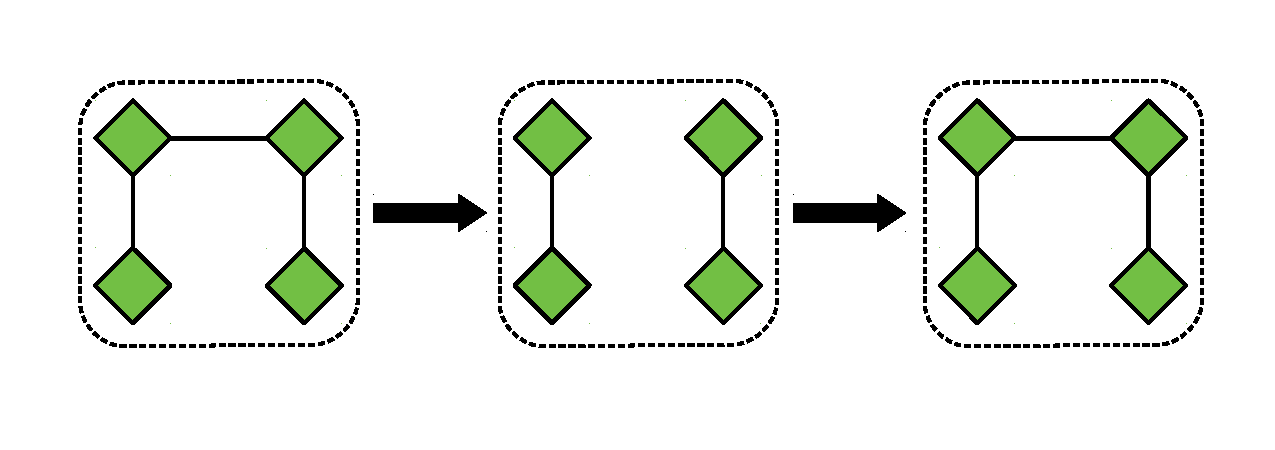
\includegraphics[width=\columnwidth]{horseshoe.pdf}
	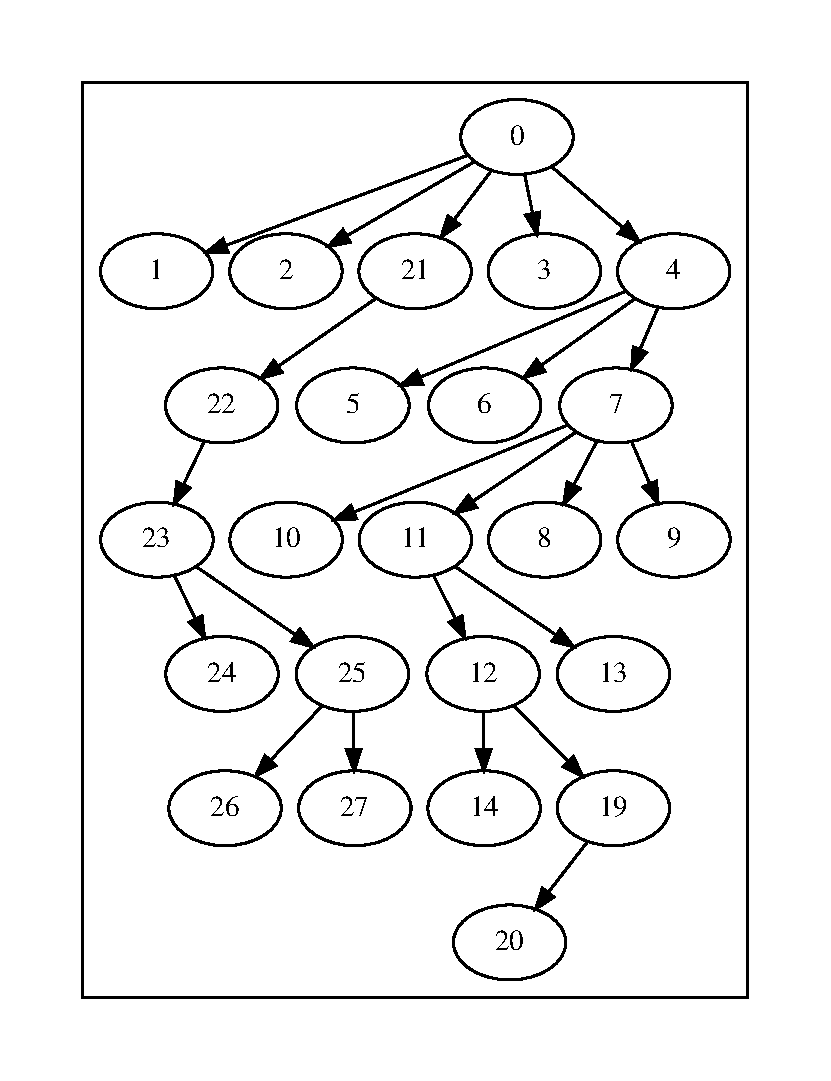
\includegraphics[width=\columnwidth]{horseshoe_0.pdf}
	\caption{A proof-of-concept SPAN-distribted blockchain simulated in SPANchain.
		The simulation is performed in the script \texttt{horseshoe\_partition.py},
		visualization of the output is performed using \texttt{make\_figures.sh}.}
	\label{fig:old_town_road}
\end{figure}


\section{Resilience against first-order attacks}

Thoughoug the entire paper,
we made the assumption that all nodes have about the same computational power.
In this section,
we consider the situation in which a single node,
without additional computational power,
is trying to disrupt the network.
That is,
we analyze the protocol's resiliency against first-order attacks.

A misbehaving node may only interfere with either the blockchain infrastructure
or with the message-passing algorithm.

Since it is not possible to erase any blocks from the blockchain,
the only way a misbehaving node could affect the ledger
is by adding blocks.
However,
as we are supposing the malicious node
has about the same computational power as the other nodes in the network,
the villain would only be able to add blocks at the same rate as the other nodes,
so these extraneous blocks would be a minority in the chain.
Distributed consensus cannot be affected by a few blocks in the chain.

For the message-passing algorithm,
the malicious node cannot forge or alter messages from other users
due to cryptographic signatures.
Dropping messages from other users is not effective;
this is tantamount to making the network disconnected,
which is a situation the protocol is designed to tolerate.

However,
the node is able to generate several extraneous cryptographic challenges;
that is,
a single node could create several virtual identities
(by generating several pairs of public and private keys)
and pose cryptographic challenges to other nodes posing as each of these identities.
Other nodes in the network would not be able to differentiate between
these virtual identities and other honest nodes,
and thus waste cycles trying to solve cryptographic challenges
posed by nodes which do not exist.
Although this attack does not erase previous blocks,
it slows down the network,
preventing it from doing meaningful progress.


\section{Conclusions and Future Work}

% TODO: Write more about simulation results

The protocol, as described in this paper,
is able to provide distributed geographical authentication
An obvious next step would be actually deploying this protocol in a real-life scenario,
to both test its reliability and compute the simulation parameters.

As outlined in Section~\ref{sec:first-order-attacks},
making the protocol resilient to first-order attacks is an open problem.
A possible solution involves adding a computational cost
to enter and stay in the network;
for example,
honest nodes could simply try to solve cryptographic challenges
from nodes which have appeared ``recently'' in the blockchain.

Another issue is that,
in the analysis,
we assume that the computational power of each node
is roughly the same.
This makes the network vulnerable to a smartphone user using,
say,
their personal computer to speed up the computation of hashes
could control the network.
A possible solution is to replace the highly parallizable hash function
with non-parallelizable cryptographic challenges~\cite{Tritilanunt2007}.


\bibliographystyle{plainurl}
\bibliography{bib}

\end{document}
